% Options for packages loaded elsewhere
\PassOptionsToPackage{unicode}{hyperref}
\PassOptionsToPackage{hyphens}{url}
\PassOptionsToPackage{dvipsnames,svgnames,x11names}{xcolor}
%
\documentclass[
  12pt]{article}

\usepackage{amsmath,amssymb}
\usepackage{iftex}
\ifPDFTeX
  \usepackage[T1]{fontenc}
  \usepackage[utf8]{inputenc}
  \usepackage{textcomp} % provide euro and other symbols
\else % if luatex or xetex
  \usepackage{unicode-math}
  \defaultfontfeatures{Scale=MatchLowercase}
  \defaultfontfeatures[\rmfamily]{Ligatures=TeX,Scale=1}
\fi
\usepackage{lmodern}
\ifPDFTeX\else  
    % xetex/luatex font selection
\fi
% Use upquote if available, for straight quotes in verbatim environments
\IfFileExists{upquote.sty}{\usepackage{upquote}}{}
\IfFileExists{microtype.sty}{% use microtype if available
  \usepackage[]{microtype}
  \UseMicrotypeSet[protrusion]{basicmath} % disable protrusion for tt fonts
}{}
\makeatletter
\@ifundefined{KOMAClassName}{% if non-KOMA class
  \IfFileExists{parskip.sty}{%
    \usepackage{parskip}
  }{% else
    \setlength{\parindent}{0pt}
    \setlength{\parskip}{6pt plus 2pt minus 1pt}}
}{% if KOMA class
  \KOMAoptions{parskip=half}}
\makeatother
\usepackage{xcolor}
\setlength{\emergencystretch}{3em} % prevent overfull lines
\setcounter{secnumdepth}{5}
% Make \paragraph and \subparagraph free-standing
\ifx\paragraph\undefined\else
  \let\oldparagraph\paragraph
  \renewcommand{\paragraph}[1]{\oldparagraph{#1}\mbox{}}
\fi
\ifx\subparagraph\undefined\else
  \let\oldsubparagraph\subparagraph
  \renewcommand{\subparagraph}[1]{\oldsubparagraph{#1}\mbox{}}
\fi


\providecommand{\tightlist}{%
  \setlength{\itemsep}{0pt}\setlength{\parskip}{0pt}}\usepackage{longtable,booktabs,array}
\usepackage{calc} % for calculating minipage widths
% Correct order of tables after \paragraph or \subparagraph
\usepackage{etoolbox}
\makeatletter
\patchcmd\longtable{\par}{\if@noskipsec\mbox{}\fi\par}{}{}
\makeatother
% Allow footnotes in longtable head/foot
\IfFileExists{footnotehyper.sty}{\usepackage{footnotehyper}}{\usepackage{footnote}}
\makesavenoteenv{longtable}
\usepackage{graphicx}
\makeatletter
\def\maxwidth{\ifdim\Gin@nat@width>\linewidth\linewidth\else\Gin@nat@width\fi}
\def\maxheight{\ifdim\Gin@nat@height>\textheight\textheight\else\Gin@nat@height\fi}
\makeatother
% Scale images if necessary, so that they will not overflow the page
% margins by default, and it is still possible to overwrite the defaults
% using explicit options in \includegraphics[width, height, ...]{}
\setkeys{Gin}{width=\maxwidth,height=\maxheight,keepaspectratio}
% Set default figure placement to htbp
\makeatletter
\def\fps@figure{htbp}
\makeatother

\addtolength{\oddsidemargin}{-.5in}%
\addtolength{\evensidemargin}{-1in}%
\addtolength{\textwidth}{1in}%
\addtolength{\textheight}{1.7in}%
\addtolength{\topmargin}{-1in}%
\usepackage{booktabs}
\usepackage{longtable}
\usepackage{array}
\usepackage{multirow}
\usepackage{wrapfig}
\usepackage{float}
\usepackage{colortbl}
\usepackage{pdflscape}
\usepackage{tabu}
\usepackage{threeparttable}
\usepackage{threeparttablex}
\usepackage[normalem]{ulem}
\usepackage{makecell}
\usepackage{xcolor}
\usepackage{xcolor}
\makeatletter
\@ifpackageloaded{caption}{}{\usepackage{caption}}
\AtBeginDocument{%
\ifdefined\contentsname
  \renewcommand*\contentsname{Table of contents}
\else
  \newcommand\contentsname{Table of contents}
\fi
\ifdefined\listfigurename
  \renewcommand*\listfigurename{List of Figures}
\else
  \newcommand\listfigurename{List of Figures}
\fi
\ifdefined\listtablename
  \renewcommand*\listtablename{List of Tables}
\else
  \newcommand\listtablename{List of Tables}
\fi
\ifdefined\figurename
  \renewcommand*\figurename{Figure}
\else
  \newcommand\figurename{Figure}
\fi
\ifdefined\tablename
  \renewcommand*\tablename{Table}
\else
  \newcommand\tablename{Table}
\fi
}
\@ifpackageloaded{float}{}{\usepackage{float}}
\floatstyle{ruled}
\@ifundefined{c@chapter}{\newfloat{codelisting}{h}{lop}}{\newfloat{codelisting}{h}{lop}[chapter]}
\floatname{codelisting}{Listing}
\newcommand*\listoflistings{\listof{codelisting}{List of Listings}}
\makeatother
\makeatletter
\makeatother
\makeatletter
\@ifpackageloaded{caption}{}{\usepackage{caption}}
\@ifpackageloaded{subcaption}{}{\usepackage{subcaption}}
\makeatother
\ifLuaTeX
  \usepackage{selnolig}  % disable illegal ligatures
\fi
\usepackage[]{natbib}
\bibliographystyle{agsm}
\usepackage{bookmark}

\IfFileExists{xurl.sty}{\usepackage{xurl}}{} % add URL line breaks if available
\urlstyle{same} % disable monospaced font for URLs
\hypersetup{
  pdftitle={Engaging students with statistics through choice of real data context on homework},
  pdfauthor={Catalina M. Medina; Mine Dogucu},
  pdfkeywords={statistics education, data science education, real
data, datasets with context, student autonomy, student interest},
  colorlinks=true,
  linkcolor={blue},
  filecolor={Maroon},
  citecolor={Blue},
  urlcolor={Blue},
  pdfcreator={LaTeX via pandoc}}


\begin{document}


\def\spacingset#1{\renewcommand{\baselinestretch}%
{#1}\small\normalsize} \spacingset{1}


%%%%%%%%%%%%%%%%%%%%%%%%%%%%%%%%%%%%%%%%%%%%%%%%%%%%%%%%%%%%%%%%%%%%%%%%%%%%%%

\date{February 4, 2026}
\title{\bf Engaging students with statistics through choice of real data
context on homework}
\author{
Catalina M. Medina\thanks{Medina has been supported by NSF IIS award
\#2123366. Medina completed an earlier part of this work in the
Department of Statistics at the University of California, Irvine.}\\
\parbox[t]{0.9\textwidth}{\centering Department of Mathematics and Data
Science}\\
\parbox[t]{0.9\textwidth}{\centering California State University Channel
Islands}\\[0.5em]
and\\[0.5em]
Mine Dogucu\thanks{Dogucu has been supported by NSF IIS award
\#2123366.}\\
\parbox[t]{0.9\textwidth}{\centering Department of Statistics}\\
\parbox[t]{0.9\textwidth}{\centering University of California,
Irvine}\\[0.5em]
}
\maketitle

\bigskip
\bigskip
\begin{abstract}
Statistics educators recommend teaching with real data with relevant
contexts, but defining relevancy is challenging and varies by student.
We investigated whether providing student choice of data context
increases engagement through a quasi-experiment in two sections of an
introductory probability and statistics course at a large public
university (n=65 consenting students). Sections alternated as treatment
and control: during their treatment, students chose weekly homework from
three similar instructor-provided options varying by data context;
during control weeks, they received randomly assigned contexts. We found
no significant difference in homework grades between treatment and
control conditions. However, thematic analysis revealed students with
choice reported enhanced engagement and motivation, greater appreciation
for statistics' real-world value, and increased autonomy. Students
overwhelmingly preferred contexts relevant to their interests,
experiences, daily lives, and career paths---though preferences varied
considerably across individuals. Based on these findings, we provide
four recommendations for statistics educators: (1) use real data with
authentic contexts, (2) select contexts students care about, (3)
incorporate variety across data contexts, and (4) consider choice as a
pedagogical tool.
\end{abstract}

\noindent%
{\it Keywords:} statistics education, data science education, real
data, datasets with context, student autonomy, student interest
\vfill

\newpage
\spacingset{1.9} % DON'T change the spacing!

\section{Introduction}\label{sec-introduction}

Among the statistics education community, there are recommendations to
use real data when teaching statistics. As Guidelines for Assessment and
Instruction in Statistics Education (GAISE) College Report
\citeyearpar{gaise2016} states in recommendation 3, instructors should
``integrate real data with a context and a purpose''. Using real data
with context helps students perceive statistics as real and relevant
\citep{neumann2013, bibby2003, brearley2018, cobb1997, cobb1992} and
engage with the discipline \citep{hall2011}. Numerous recommendations
exist on how to teach with real data and where to find it
\citep{hall2011, singer1990}. We believe statistics should be taught as
an investigative tool to learn from data about the world.

We present Table~\ref{tbl-data-types} to clarify what we mean by real
data with a context. \emph{Made up data} is artificially created and
easiest for instructors to generate but provides no real information.
\emph{Empirically informed data}, data simulated from real statistics or
parameter estimates, mimics real phenomena but cannot provide reliable
real-world implications. \emph{Real data} is generated from real-world
events or observations. Often we tailor real data to demonstrate
specific concepts by dropping data points, but this can remove meaning
since data no longer reflects what actually occurred. We distinguish
tailoring from cleaning, where cleaning converts data to readily usable
form. Real raw data provides exposure to data encountered in real
practice but may require substantial wrangling. Regardless of data type,
without context there is no information to be gained from statistical
analysis. This work focuses on real cleaned data with context.

\begin{table}

\caption{\label{tbl-data-types}Data context types with some pros and
cons identified.}

\centering{

\centering
\begin{tabular}[t]{>{\centering\arraybackslash}p{1.6 in}>{\centering\arraybackslash}p{0.7 in}>{\centering\arraybackslash}p{0.7 in}>{\centering\arraybackslash}p{0.7 in}>{\centering\arraybackslash}p{0.7 in}>{\centering\arraybackslash}p{0.7 in}}
\toprule
\multicolumn{4}{c}{ } & \multicolumn{2}{c}{Real-world implications} \\
\cmidrule(l{3pt}r{3pt}){5-6}
Data Type & Easily Obtained & Readily Usable & Realistic Practice & With Context & Without Context\\
\midrule
\cellcolor{gray!10}{Simulated (made up)} & \cellcolor{gray!10}{$\checkmark$} & \cellcolor{gray!10}{$\checkmark$} & \cellcolor{gray!10}{} & \cellcolor{gray!10}{} & \cellcolor{gray!10}{}\\
Simulated (empirically informed) & $\checkmark$ & $\checkmark$ &  &  & \\
\cellcolor{gray!10}{Real (tailored)} & \cellcolor{gray!10}{} & \cellcolor{gray!10}{$\checkmark$} & \cellcolor{gray!10}{} & \cellcolor{gray!10}{} & \cellcolor{gray!10}{}\\
Real (cleaned) &  & $\checkmark$ &  & $\checkmark$ & \\
\cellcolor{gray!10}{Real (raw)} & \cellcolor{gray!10}{} & \cellcolor{gray!10}{} & \cellcolor{gray!10}{$\checkmark$} & \cellcolor{gray!10}{$\checkmark$} & \cellcolor{gray!10}{}\\
\bottomrule
\end{tabular}

}

\end{table}%

When an instructor decides they want to use real data, the natural
question is what real data contexts should they use? Many are of the
opinion that the data we should engage students by using data relevant
to their everyday lives. Even once an instructor decides they want to
use real data with a context relevant to their students' daily life,
there is the challenge of deciding what is relevant to their students.
\citet{sole2017} used data about coffee sales and \citet{gould2010}
recommends using data about music, social media, maps, exercise, and
data from personal devices. \citet{gunderman2020} proposed using popular
culture to engage learners in spatial data management skills, with
examples applied to topics learners typically see as uninteresting.
\citet{ludlow2002} proposed using data from the instructor's own faculty
evaluations to engage students. \citet{brooks2021} tried to achieve
relevance in their massive open online course by using weather data from
the student's region of residence, but their findings led them to
suggest using data relevant to the students' career identities instead.
In addition to recommending data relevant to students' daily life,
\citet{neumann2013} also recommended using data relevant to a student's
major. \citet{brearley2018} discuss using research articles relevant to
students' fields. Using data relevant to students' career goals may help
bridge the gap between what teachers perceive as relevant to a student's
life and what the student perceives as relevant. This recommendation
would be helpful in classes where students are from the same or similar
majors, but less helpful in class with students from a diverse set of
majors.

Despite the efforts of teachers to find data with compelling context,
not every student will engage with every data context. Therefore there
are recommendations to use a diverse set of real data contexts
\citep{gaise2016}, with effort made to engage students with some subsets
of the data contexts investigated in the course. Alternatively, some
suggest engaging students with real data by using data collected on the
students. \citet{schneiter2023} suggests that large class sizes may be
especially posed to benefit from data collection on students by
demonstrating concepts like sampling distributions in addition to
engaging students. \citet{hulsizer2009} investigated the importance and
psychological pros and cons of using data collected on your students.

Another pathway is allowing students to choose data contexts, either in
assignments \citep{boger2001} or projects \citep{cetinkaya-rundel2022}.
\citet{boger2001} compared effects by having one section investigate
instructor-provided data while another had free choice across four
assignments. Interestingly, students given autonomy reported
significantly decreased perceived usefulness of statistics in their
field. \citet{boger2001} posed this decrease could be due to increased
effort required for students to choose and collect their own data.

While there have been many recommendations of data contexts to use there
is little empirical evidence for certain contexts over others. Even
among the common recommendation of using data relevant to students,
there is little systematic study of what data students find as relevant
to themselves. One thing our study sought to answer is: what do our
students perceive as relevant to themselves, and why? Investigating this
question can provide ideas and support for what could be relevant to
your students. More broadly, we hoped to investigate preference and
impact of student-chosen data context to better understand what data
contexts we should be selecting as an instructor, why it may or may not
be worth the effort, and if we should give students some autonomy in
selection of context.

We hypothesized that students having the autonomy to choose the data
context that they would like to work on from multiple data contexts
provided to them, may lead students to be more engaged with the
material. We investigated this through a quasi-experiment. In one
section of a course we allowed students to choose their weekly homework
assignment from three similar instructor-provided options that varied by
the data context, while the other course section did not receive a
choice. This investigation of choice of data context was implemented at
a large public institution in two sections of an undergraduate
introductory probability and statistics course taught by a single
instructor. As statistics and data science instructors we wanted to
learn if we should provide students choice of data context and what data
contexts should we be choosing for students? In this work we
investigated if given the choice between similar homework assignments
that differ by data context (1) do students achieve higher grades
relative to students not given choice, (2) how do students perceive
having a choice of data context, (3) what characteristics of the data
contexts led students to choose one option over the others?

\section{Methods}\label{sec-methods}

\subsection{Study setting}\label{study-setting}

The quasi-experiment was implemented in two sections of an undergraduate
class at a large public research university in winter of 2025. The class
was an introduction to probability and statistics course mainly for
computer science majors, totaling 180 active students across the two
sections. The first half of the class was mainly an introduction to
probability, while the last half of the ten-week course was mainly an
introduction to statistics, the intervention period. The only
prerequisite to the course was a single-variable calculus course. 65
students provided consent for their data to be used for research
purposes, 33 from section A and 32 from section B. The students were not
provided any incentive to participate (e.g., extra credit or monetary
compensation), and were informed that their professor would not know who
consented to be part of the study until after final grades were
submitted.

For each week of the quasi-experiment each student in the treatment
section was able to choose between three options of similar homework
assignments, varying mainly by data context investigated in the
homework. The students in the control section were not given options,
and were instead randomly assigned one of the three context options that
the treatment section received. It was randomly assigned which section
of the class would receive the treatment, choice between assignments,
for the first two weeks of the intervention period. For the last two
weeks of the intervention period the treatment and control were swapped,
so each section would ultimately experience two weeks of the
intervention and two of the control, see
Table~\ref{tbl-experimental-design}.

\begin{table}[!htb]

\caption{\label{tbl-experimental-design}Data context quasi-experimental
design.}

\centering{

\centering
\begin{tabular}[t]{>{\raggedright\arraybackslash}p{2cm}>{\raggedright\arraybackslash}p{5cm}>{\raggedright\arraybackslash}p{5cm}}
\toprule
\multicolumn{1}{c}{ } & \multicolumn{2}{c}{Data context choices} \\
\cmidrule(l{3pt}r{3pt}){2-3}
Week & Section A & Section B\\
\midrule
\cellcolor{gray!10}{1} & \cellcolor{gray!10}{Cheating with AI\newline Gluten-free pasta\newline Home-team advantage} & \cellcolor{gray!10}{Cheating with AI}\\
2 & Cheating with AI\newline Electric vehicle adoption\newline Sleep deprivation & Sleep deprivation\\
\cellcolor{gray!10}{3} & \cellcolor{gray!10}{Typing speeds} & \cellcolor{gray!10}{Dog lifespans\newline Teen pregnancies\newline Typing speeds}\\
4 & 2003 movies & 2003 movies\newline Bike shares\newline Gorillas\\
\bottomrule
\end{tabular}

}

\end{table}%

Each homework assignment was centered around one real data set, with
context provided to motivate the research questions investigated. All
surveys and assignments were integrated as part of the curriculum and
are available in the Supplemental Materials.

We intentionally chose the data contexts each week to at minimum be
contexts we thought could interest students and covered a variety of
disciplines each week. There were some additional context
characteristics we wanted to investigate including: serious vs
lighthearted (i.e., teen pregnancy vs typing speed), older (i.e., 2003
movies), scientific studies unrelated to humans (i.e., gorillas), and
recycled contexts (i.e., cheating with AI).

\subsection{Homework centered around real data with
context}\label{homework-centered-around-real-data-with-context}

Each homework assignment was centered around the investigation of a real
data set with context. The homework assignments were computer-based
where the student would either see one homework or three homework
options for that week, with the statistical topic and data context
included in the title when choice was provided. For example,
intervention week one a student with choice of data context would see:
``hw6-single-prop-cheating-with-AI'',
``hw6-single-prop-gluten-free-pasta'', and
``hw6-single-prop-home-team-advantage''.

The data context was included in the title so students would immediately
be aware of the data context, even without opening the assignment. The
assignments where students were given a choice began with ``Note: There
are three options for homework {[}number{]}, that differ by data topic,
and you only need to complete one of the three assignments''. Within the
assignment there would be a brief introduction to the data context with
either the data file, or a link to the study it came from. For example,
the sleep deprivation homework option of intervention week 2 began:

``Sleep deficiency can affect your physical, cognitive, and social
functions. Sleep deprivation has been linked to many chronic health
problems including obesity and depression. The CDC conducted a study in
2008 {[}link embedded{]} to investigate sleep deprivation among United
States residents\ldots{}''

The homework would involve an investigation of the real data within
context, with questions consistent across homework options for that week
that only varied by data context. For example, for two intervention
homework 2 options, question 2 began either:

\begin{quote}
``We want to calculate a 90\% CI for the difference in proportion of
residents that experienced sleep deprivation for the past 30 days
between California and Washington\ldots{}''
\end{quote}

\begin{quote}
``We want to calculate a 90\% CI for the difference in proportion of
public high school students that used a digital device as an
unauthorized aid between 2019 and 2023\ldots{}''.
\end{quote}

The real data investigation would sometimes be supplemented by
hypothetical questions within the context, but with artificial numbers
to have students explore theoretical properties, such as what happens to
the standard deviation when sample size increases.

\subsection{Data collection and
analysis}\label{data-collection-and-analysis}

\textbf{Research question 1: do students achieve higher grades relative
to students not given choice?} First, we wanted to detect if there were
differences in weekly homework grades associated with being given a
choice of data context? We had access to all of the students homework
grades, including those before the intervention period. Specifically, we
chose to look for differences in a students homework grade relative to
their average pre-intervention period homework grade, associated with
having a choice of data context. We chose to investigate this with a
generalized estimating equation where the response for student \(i\) at
time \(t\) was regressed on whether they had a choice of data context
for the homework, the student's section, and separate indicators for
intervention week. An exchangeable correlation structure was used for
each student to control for intra-student correlation across time
points. \begin{equation}\phantomsection\label{eq-hw}{
\begin{split}
&\text{Intervention Homework Grade}_{it} - \text{Average Pre-intervention Homework Grade}_{i}\\
&= \beta_0 + \beta_1 {I_{(\text{Choice})}}_{it} + \beta_2 {I_{(\text{Section B})}}_{i} + \beta_3 {I_{(\text{Week 2})}}_{t} + \beta_4 {I_{(\text{Week 3})}}_t + \beta_5 {I_{(\text{Week 4})}}_t + \epsilon_{it}
\end{split}
}\end{equation}

\textbf{Research question 2: how do students perceive having a choice of
data context?} We surveyed students after the intervention period to
answer research question 2. We asked ``What did you think about having
three homework assignment options to choose from that differed by data
context for two homework assignments in this class?'', since each
section only had choice of data context for two weekly homework
assignments. From students responses to this question, we qualitatively
identified themes and judged if the students opinion seemed to be
overall negative, impartial, or positive.

\textbf{Research question 3: what characteristics of the data contexts
led students to choose one assignment over the other options?} The
second goal of this work was to investigate why students chose a data
context over the other options, and what they did or did not like about
a given data context. At the end of each homework assignment the
students had a question related to the data context, which varied
depending on whether the student had a choice of data context for that
assignment. Consider intervention homework 1 and the cheating with AI
topic, which was the randomly assigned topic for section B.

The students not given a choice of data context (section B) were asked:

\begin{itemize}
\tightlist
\item
  ``Please explain in detail what you liked and/or what you did not like
  about this data topic''
\end{itemize}

Students given a choice of data context (section A) were asked:

\begin{itemize}
\tightlist
\item
  ``Please explain in detail what led you to choose this topic, cheating
  with AI, to investigate'' and
\item
  ``What was it about the other two options (gluten-free pasta and
  home-team advantage) that led you not to choose them? Please explain
  in detail''
\end{itemize}

These questions also specified that there were no correct answers and
these questions were only being graded for completeness. Thematic
analysis was used to identify reoccurring themes among the students'
responses to these questions, both researchers independently identified
a theme, or multiple themes, for each student's response to the data
context question(s) \citep{braun2006}. The themes were recorded as
either being specific to a context, or nonspecific to the context (e.g.,
the student just chose the first homework option on the screen). The
researchers then resolved any conflicts together. Due to technical error
we did not have this data from the no choice section (section A) in
intervention week 3.

\section{Results}\label{results}

Analysis of surveys and homework revealed four overarching categories
related to having choice of real data context: (1) students' sentiment
about having choice, (2) student perceived qualitative outcomes, (3)
quantitative outcomes, and (4) students' desired characteristics of real
data context.

\subsection{Students' sentiment about having
choice}\label{students-sentiment-about-having-choice}

From the post-survey we judged 2 students to have an overall negative
opinion, 18 overall impartial opinions, and 43 students to have an
overall positive of having a choice of data context.

The two students with an overall negative opinion thought having a
choice ``added unnecessary difficulty'' or ``made starting the
assignment a little harder since I had to decide which topic to pick.''
This indicated that the students somewhat cared about which homework to
pick, but unfortunately they thought the ``options were still a bit
limited.'' While only two students had overall negative opinions, there
were two more comments about negative aspects of having choice. A couple
students expressed having their peers working on different assignments
made ``it more difficult to discuss the best way to solve certain
problems'' or ``understand the concepts if they work on differing
work.'' Another student expressed the opposite opinion on the situation
stating ``I do like that having variety means that it's not as easy to
copy answers from other students.''

Most of the students that had overall impartial opinions expressed that
having a choice of data context had no effect on them. Some even
specifically said it ``didn't make my homework more or less enjoyable''
or ``they provide no significant benefit to my learning of the course
topics.'' A few students expressed disinterest in the offered topics,
with one saying ``the topics would only matter to me if they were
actually interesting to me, and if they're just three random topics that
all equally are not that interesting to me then there's no point for
me.'' One student even said ``the context of the analysis wasn't as
useful as the actual data was'', which is the opposite of the
instructor's goal of working with real data with a real context on the
homework. A student that was overall impartial did acknowledge that
while they were ``ambivalent on the matter\ldots{} I do think that it
could benefit some students''.

Among all sentiments there were students that simply appreciated having
autonomy, regardless of what that autonomy pertained to. ``I really
liked having the ability to choose. That small privilege somewhat made
the homework more pleasing.'' One student even expressed ``I found it
more interesting when I got to choose perhaps that's the illusion of
choice.'' A couple of students pointed out that having multiple options
for homework assignments provided opportunities for further studying and
practice with the assignments they did not choose.

Many of the students that expressed an overall positive sentiment
described experiencing some qualitative outcome resulting from having
choice of data context, which will be discussed in detail in the
following section.

\subsection{Qualitative outcomes}\label{qualitative-outcomes}

While we did not intend to investigate any associations with our
intervention other than grade differences, thematic analysis revealed
many themes of students identifying positive experiences. The following
is an exemplary response:

\begin{quote}
\emph{I thought that having more options on what context to do problems
with was pretty interesting overall, and helped motivate me to do the
homework knowing that there was a tangible and significant reason for
doing it. By that I mean that doing the homework to solve a problem I'm
interested in seems more like something I would want to do on my
off-time than something done for a grade, so I was more engaged in the
assignment.}
\end{quote}

We classified students' responses as being associated with working with
real data from a real context, working with real data from a context
students are interested in, and working with real data from a context
students are interested in and chose themselves, visualized in
Figure~\ref{fig-perceived-positive-outcomes}. It is important to note
that we had a low consent rate, so identified themes not necessarily
representative of all of the students in the class, but we can still
learn from the themes that consistently emerged.

\begin{figure}

\centering{

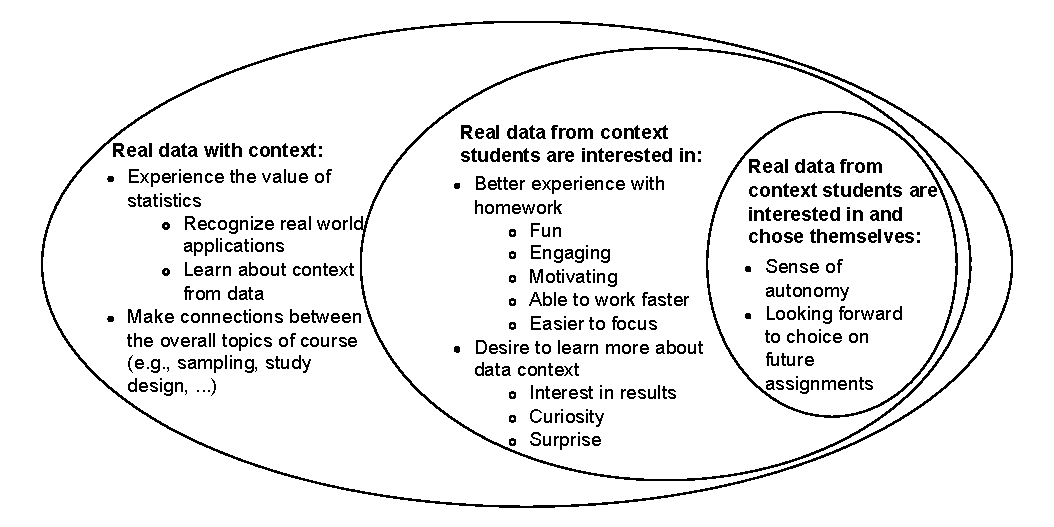
\includegraphics[width=6in,height=3in]{figures/perceived-outcomes.pdf}

}

\caption{\label{fig-perceived-positive-outcomes}Students' perceived
positive outcomes.}

\end{figure}%

As a student expressed, when working through an assignment using real
data with context ``statistics homework will let the student get more
insight on the topic.'' Even more it ``showed that statistics is not
just some hypothetical numeric calculation, but rather something that
could actually have real-world impacts.'' Instead of instructors arguing
why statistics is useful, students were reporting that they experienced
it being useful. Furthermore, some students were even thinking beyond
the homework questions discussing considerations of a study's design or
concerns of bias due to sampling scheme. ``It was cool to see survey
results showing whether students admit to using AI. I just wish the
sample sizes were bigger so we'd be more confident in the findings.''
Having a real context provides depth for students to apply all of their
statistical knowledge, not just the content they learned that week.

More benefits were identified when the data was not only real with
context, but specifically from a context students were interested in
``Rather than looking at the probabilities of flipping heads or rolling
a die, I enjoyed learning through this example because it has a greater
real-life impact.'' Students often expressed this led to the homework
being more fun, engaging, and or motivating, with some saying they were
able to work faster and or had an easier time focusing. A desire to
learn more about the data context was expressed both in why they chose a
context and in their discussion of the results they found in the
homework. ``I have a large dog at home who I love A LOT. I can never
think about his lifespan and only wish for him to live forever. However,
I chose this study in hopes of understanding more about the topic.'' At
the end of homework assignments when we asked why they did or didn't
choose certain contexts, several students used this as an opportunity to
further describe or explore the results they found. They reasoned
whether or not the results made sense to them given their knowledge or
experience, articulated surprise at unexpected patterns, posed possible
explanations for findings, and one looked into unused variables in the
data to explore more associations.

The innermost ring of Figure~\ref{fig-perceived-positive-outcomes}
highlights the positive outcomes associated with students being able to
choose their context. Providing a choice of context was not only a
mechanism to increase chances of students working with a context they
are more interested in. Students said the autonomy itself ``\ldots{}
allowed us to express some creativity and independence of choice'' and
another said ``that small privilege somewhat made the homework more
pleasing.'' One person said knowing they would have a choice made them
look forward to their next assignment.

\subsection{Quantitative outcomes}\label{quantitative-outcomes}

Using the model described in Equation~\ref{eq-hw} we did not find
evidence of a difference between a student's homework score relative to
their average homework scores pre-intervention (p-value = 0.2377).
Further model results are available in the Table S1. While lack of
effect of choice could possibly explain these results, we also note they
could also be due to other factors such as low statistical power or a
misspecified model. We chose an exchangeable within student covariance
structure to account for within student variation and the limitation of
our small sample size. A better option may be to account for expected
difference in correlation between the two treatment homework assignments
and between the two control homework assignments, if there was more
statistical power. Finally, a challenge of modeling homework grades is
the ceiling effect. Any theoretical improvement from an already near
perfect scoring student would be near unobservable depending on how
close the score is to the maximum.

\subsection{Students' preferred real data context
characteristics}\label{students-preferred-real-data-context-characteristics}

\begin{figure}[!htb]

\centering{

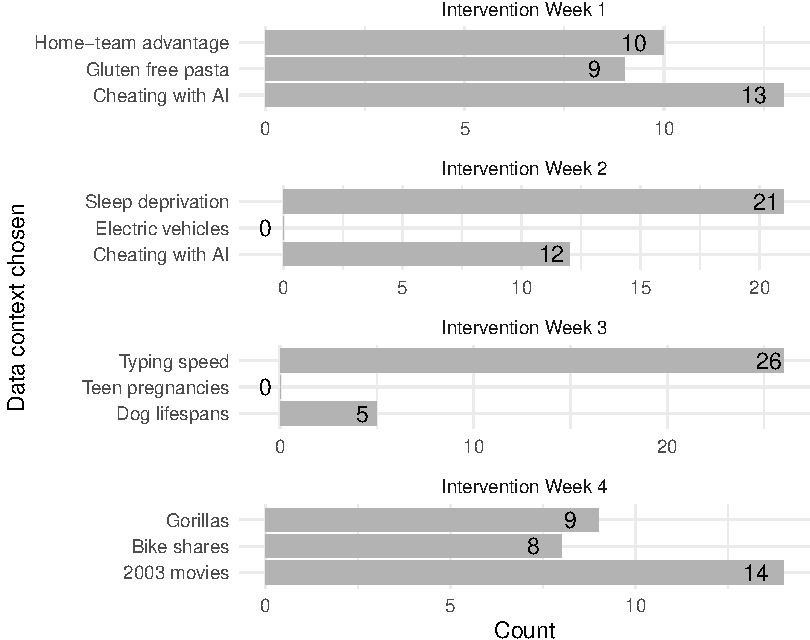
\includegraphics{00-manuscript_files/figure-pdf/fig-chosen-contexts-1.pdf}

}

\caption{\label{fig-chosen-contexts}Number of students that chose each
data context by week, among students given choice of data context.}

\end{figure}%

Figure~\ref{fig-chosen-contexts} displays the counts of how many
students chose a given data context, among lecture A students for the
first two intervention weeks and lecture B students for the last two. No
student chose electric vehicles in intervention week 2 or teen
pregnancies in week 3. Additionally, very few students chose dog
lifespans in week 3.

Themes of why students chose certain contexts and not others are
summarized in Figure~\ref{fig-desirable-data-context-characteristics}.
Two major takeaways are that students have conflicting opinions and they
overwhelmingly prefer contexts that are relevant to them and have some
previous knowledge of.

\begin{figure}

\centering{

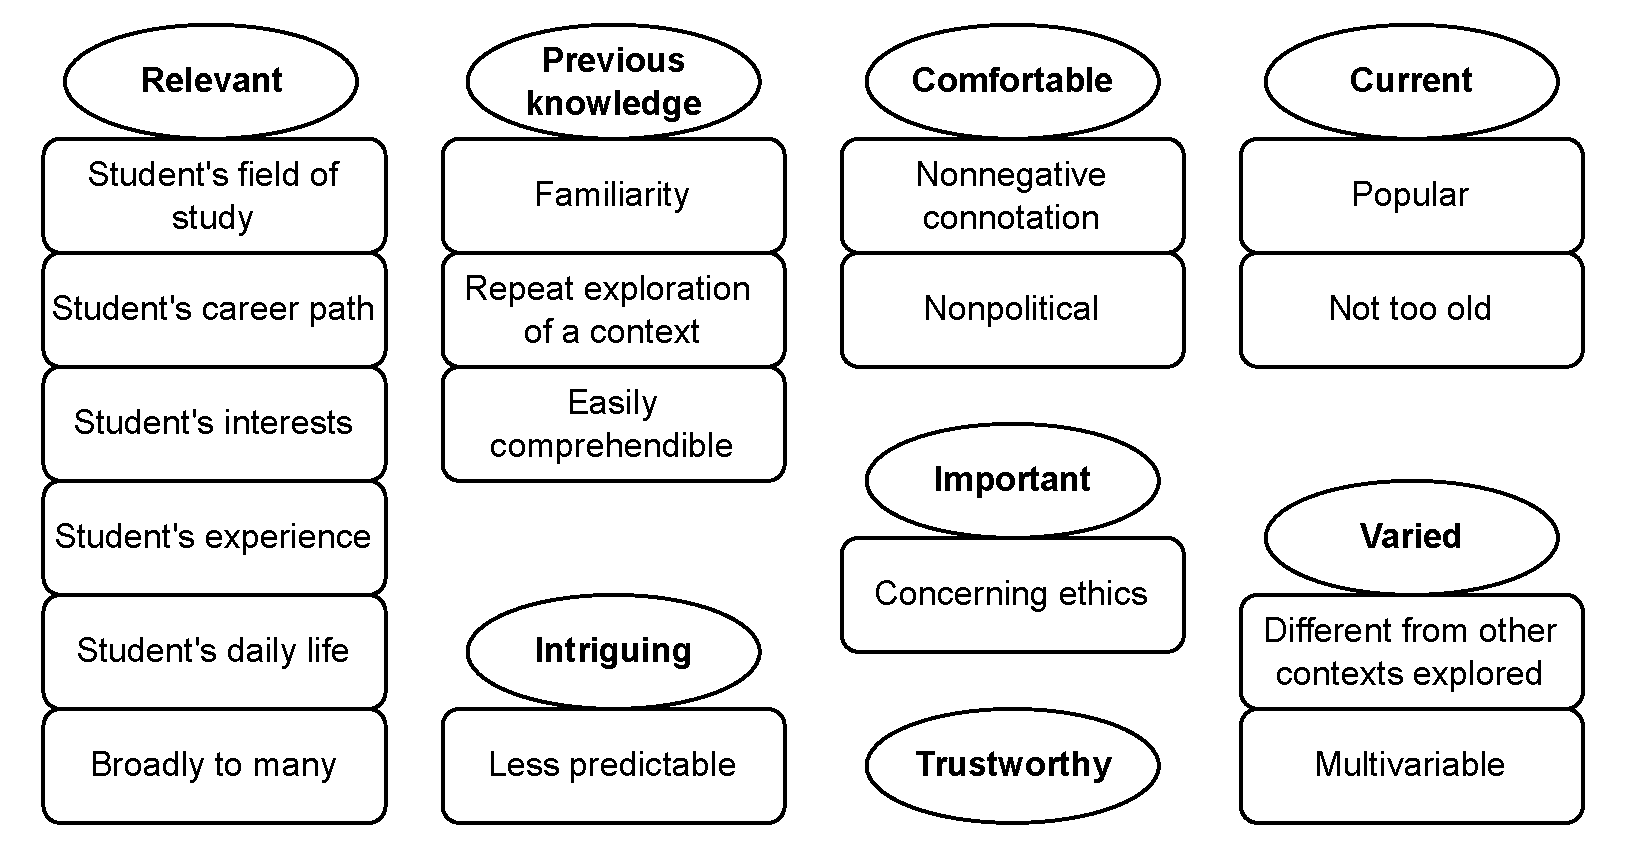
\includegraphics[width=6in,height=3in]{figures/desirable-data-context-characteristics.pdf}

}

\caption{\label{fig-desirable-data-context-characteristics}Desirable
data context characteristics expressed by students.}

\end{figure}%

To the first point, some students liked a topic because they felt it was
important or commonly discussed, while others disliked it for those very
reasons. Some students chose the AI topic the second week because they
had chosen it for the first topic, but other students either didn't like
the context in the first place or preferred learning about a variety of
contexts. Some students found the 2003 movies data to be too old because
it was from around or before they were born while others preferred the
dataset because they liked movies more than they cared about them being
old.

People caring more about things that are relevant to them is not a new
idea, but relevance can be very difficult to identify for an instructor.
Students' responses help provide more specify ways they identified a
context to be relevant such as their field of study, career path,
interests, experience, daily life.

Some preferences were less obvious, such as liking a context because
they did not know what the results were likely to be beforehand or not
liking a context because they felt a lack of trust in the quality of the
data inherently due to the topic. This one arose primarily from the
cheating with AI topic where students assumed there would be under
reporting. Another less commonly discussed preferred characteristic was
for richer data where they can look further into associations beyond
what was explored in the homework.

\section{Discussion}\label{sec-discussion}

\subsection{Recommendations for statistics and data science
educators}\label{recommendations-for-statistics-and-data-science-educators}

\textbf{Recommendation 1: Use real data with a real context}\\
\underline{Why?} A major theme we identified was students wanting to
learn about the data context through the assignment, or expressing
interests in the results of the analysis. This is not possible without
real data from a real context, and artificial data from a real context
may just perpetuate the perception of statistics being fake or made up.
Our findings in support of the use of real data with a real context are
in line with the empirical findings of \citet{neumann2013} and the
recommendations of many in the literature, including the
\citet{gaise2016}.

\underline{How?} We believe statistics and data science should be taught
with real data generally, but we are not arguing against the use of
simulated data when appropriate. Simulated data can be very helpful for
exploring theoretical properties and ideas. We are arguing against the
use of artificial data in place of real data, especially when the
argument is just that using artificial data is easier for the
instructor. To facilitate this we provide a list of resources we have
found useful for finding data sets for educational purposes, available
in the Supplementary Materials .

\textbf{Recommendation 2: Use data contexts students care about}\\
\underline{Why?} \citet{neumann2013} found a common theme of students
finding the use of real data being engaging and motivating, and we
additionally found empirical evidence of students being further engaged
and motivated by real data with data contexts they were interested in.
Improving students' experiences when learning statistics is a great
motivator for instructors to strive to include interesting data set for
students.

Contrary to \citet{young-saver2024}, while we did not find a change in
quantitative outcomes, we did have a lot of students saying they had a
better experience with their homework when they were more interested or
familiar with a topic. Even though there were also many students that
did not feel choice of data context made any difference in their
experience, we still think that being able to better engage some
students is worth the effort.

\underline{What?} We found several themes among students' data context
preferences that can help us learn what students care about. Students
preferred data that was relevant to them, their experiences, daily lives
or lives as students, and their academic, career, and personal
interests.

Many students avoided the dog lifespan and teen pregnancy topics,
perceiving them as negative or challenging. The dog lifespan context
inherently involves death, so we don't feel this was a misunderstanding.
However, we believe we inadequately introduced the teen pregnancy topic,
resulting in an unintended perception. When working with sensitive or
uncomfortable topics, it's important to be extra conscious of how we
introduce the data context to students.

\underline{How?} Students often associated familiarity with a topic with
easier homework. Instructors should introduce data contexts before
expecting students to engage with data. When introducing concepts
students struggle with, use familiar and easily understood data contexts
to reduce the burden of simultaneously understanding both the concept
and the context.

We believe that statistics can fuel a love of science, but scientific
studies can be intimidating for both instructor and students to
understand and they run the risk of being perceived as ``just numbers''.
\citet{evans2023} recommended using a study on human-dog interaction as
a more accessible option for increasing engagement in undergraduate
statistics courses. Other scientific studies can be made accessible by
introducing them in ways connected to students. For example, we may want
to use the study ``Microbiome of Clothing Items Worn for a Single Day in
a Non-Healthcare Setting'' because it is relatively accessible with only
basic statistics used \citep{whitehead2023} and can be made relevant to
students by asking ``Think about wearing your clothes all day and then
sitting in your bed with them, what bacteria or fungus has
accumulated?''. \citet{singer1990} proposed using local dissertations as
a way to involve real data relevant to students. This could help
demystify the intimidating topics of scientific research, graduate
school, and dissertations while helping students see what their own
institution is contributing to society.

Another way to provide students data with contexts they care about is to
ask them through a survey \citep{weiland2024}, or even collect data on
the students themselves to use in class \citep{schneiter2023}. From this
feedback a few datasets used in the class could be selected for
substitution.

We do not recommend relying solely on our own perceptions of what
students will care about. Anecdotal evidence supporting this: both
investigators predicted which data contexts would be most chosen and
were wrong every week. Despite working with our student population for a
while, we were severely incorrect about their preferences. Instead of
choosing data based on our own opinions, we can be more successful by
listening to what students say they care about.

\textbf{Recommendation 3: Teach with a variety of data contexts}\\
\underline{Why?} No single data context appeals to all students, so
limiting contexts reduces engagement opportunities. Preferences change
over time and between classes---even some computer science majors found
the cheating with AI dataset extremely boring. While we cannot make
everyone happy, variety helps us reach more students throughout the
course. Students working with different contexts were able to see how
statistics is meaningful and applicable to real-world problems. We want
students to see that the same statistical methods are useful across many
different contexts, not just one.

\underline{How?} Reflecting on data contexts used throughout your course
can help assess variety. Getting data from diverse sources helps prevent
contexts from being too similar.

In addition to incorporating different contexts, providing rich datasets
with multiple variables can help engage students. The 2003 movies
dataset was most popularly chosen in the last week, with students
commenting about movies they examined or relationships they investigated
outside the assignment scope---they went out of their way to engage with
the data. \citet{gaise2016} recommends engaging students with
multivariable thinking; we can achieve this objective and encourage
students' curiosity by providing rich datasets they want to explore.

\textbf{Recommendation 4: Consider choice as a pedagogical tool}\\
\underline{Why?} Even though we provided a variety of data sets, we
still had students that were sometimes not intrigued by any of the
options. By providing students with choices of data context, we can
accommodate different interests at the same time, instead of only
engaging each student a few times throughout the course. Additionally,
students appreciate having autonomy, even for small tasks like choosing
between similar homework assignments. It also provides students with
more resources to practice the material beyond the required assignments.
As discussed in the introduction, some instructors provide choice of
data context through a final project. Alternatively, by providing some
choices throughout the course we can hopefully engage more students
before the end of the course. A consideration to be aware of is when you
want all students to interact with a certain data context, versus when
you are okay with them having a choice.

\underline{Why not?} We recognize that it may not be feasible for all
instructors or for all assignments. Beyond the initial burden of finding
and incorporating multiple real data sets with contexts we think
students will care about, there is also the struggle of grading
different assignments. The burden of finding data can be tackled across
multiple iterations of a course, but the burden of grading assignments
should be taken into consideration.

\subsection{Limitations and future
directions}\label{limitations-and-future-directions}

This study was for choice with homework assignments, so we do not know
if these findings would necessarily be the same for projects. Also, we
always provided 3 options, but purposely did not give them free choice.
We do not know what is the ideal number of choices to provide students
to balance variety for students with feasibility for instructor.

Future investigations could build on this work by researching these
questions on a larger scale and refining the questions we use to collect
students opinions about their experience. Separating our questions to
tease out more explicitly students' opinions on (1) having choice of
data context; (2) context characteristics preference; (3) and their
experience with their homework due to having a choice, could provide a
clearer understanding of the benefits or challenges distinct to each
component.

Our sample was limited by being a major specific course taught by a
single professor and the random assignment of treatment was done by
section not at an individual level, so it was only a quasi-experiment.
The low consent rate of the students and having a non-representative
sample prevent us from generalizing our results broadly. This was only
an initial investigative study and will require further investigation,
but our identified themes provide empirically supported avenues for
future targeted investigations.

\newpage

\section*{References}\label{references}
\addcontentsline{toc}{section}{References}

\renewcommand{\bibsection}{}
\bibliography{references.bib}




\end{document}
